
\documentclass{ar-1col}

\usepackage{amsmath, amsfonts}
\usepackage[comma]{natbib}
\usepackage{url}
\setcounter{secnumdepth}{4}

% Metadata Information
\jname{Xxxx. Xxx. Xxx. Xxx.}
\jvol{AA}
\jyear{2020}
\doi{10.1146/((please add article doi))}



\begin{document}

% Page header
\markboth{Hassan and Zhang}{The Economics of Currency Risk}

% Title
\title{Title: Subtitle}


% Authors, affiliations address.
\author{Tarek A. Hassan,$^1$ and Tony Zhang$^2$ \affil{$^1$Department of Economics, Boston University, Boston, USA, 02213; email: thassan@bu.edu} \affil{$^2$Board of Governors of the Federal Reserve System, Washington, USA, 20551; email: tony.zhang@frb.gov}}



\title{The Economics of Currency Risk \thanks{The views in this paper are solely the responsibility of the authors and should not be interpreted as reflecting the views of the Board of Governors of the Federal Reserve System or any other person associated with the Federal Reserve System.}}



\begin{abstract}
  This article reviews the literature on currency and country risk with a focus on its macroeconomic origins and implications. A growing body of evidence shows countries with safer currencies enjoy persistently lower interest rates and a lower required return to capital, and accumulate relatively more capital than countries with currencies international investors perceive as risky. Whereas earlier research focused mainly on the role of currency risk in generating violations of uncovered interest parity and other financial anomalies, more recent evidence points to important implications for the allocation of capital across countries, the efficacy of exchange rate stabilization policies, the sustainability of trade deficits, and the spillovers of shocks across international borders.
\end{abstract}


% Keywords, etc.
\begin{keywords}
  currency risk, country risk, capital flows, uncovered interest parity, carry trade, forward premium puzzle
\end{keywords}
\maketitle

% Table of Contents
% \tableofcontents

\section{Introduction}


A key tenet in economics is that the degree to which firms should be willing to invest in a given project depends crucially on the required rate of return to capital: A price-taking firm should install just enough capital for its marginal product of capital, $MPK_i$, to equal the required rate of return to capital, $r_i$,
\begin{equation}
  MPK_i=\underbrace{r^f+RP_i}_{r_i}.
  \label{eq_one}
\end{equation} 
This equation is the point of departure for many classic questions in economics. Students of asset pricing are taught that a firm's $r_i$ has two components: a risk-free part, $r^f$, and a risk premium, $RP_i$, that depends on the firm's risk characteristics. One of the classic puzzles in asset pricing asks why $RP_i$ is so large relative to $r^f$ (the equity premium puzzle). Monetary economists are interested in a central bank's power to increase or decrease investment by manipulating $r^f$, whereas students of economic growth often take differences in $MPK_i$ as a measure of inefficiencies in the allocation of capital across countries, sectors, and firms.

In this article, we argue that recent insights from the study of currency risk premia have important lessons for how we should think about equation \ref{eq_one}, and by extension, for its key applications in asset pricing, macroeconomics, and economic growth. The simplest, and perhaps most important, of these lessons is that countries differ dramatically in their risk-free interest rates. These differences in risk-free interest rates are large (on the same order of magnitude as the equity premium puzzle), appear to be highly persistent over time (lasting for decades rather than years), and cannot be explained by predictable depreciations, government default, or differences in inflation rates. Instead, these differences in interest rates appear intimately linked to the risk characteristics of the country's exchange rate and to its exchange rate regime.

\begin{figure}[htp!]
  \centering
  \caption{New Zealand Dollar vs. Japanese Yen}
  \label{fig:fp}
  \label{fig:spot}
  \begin{minipage}[htp]{0.49\textwidth}
  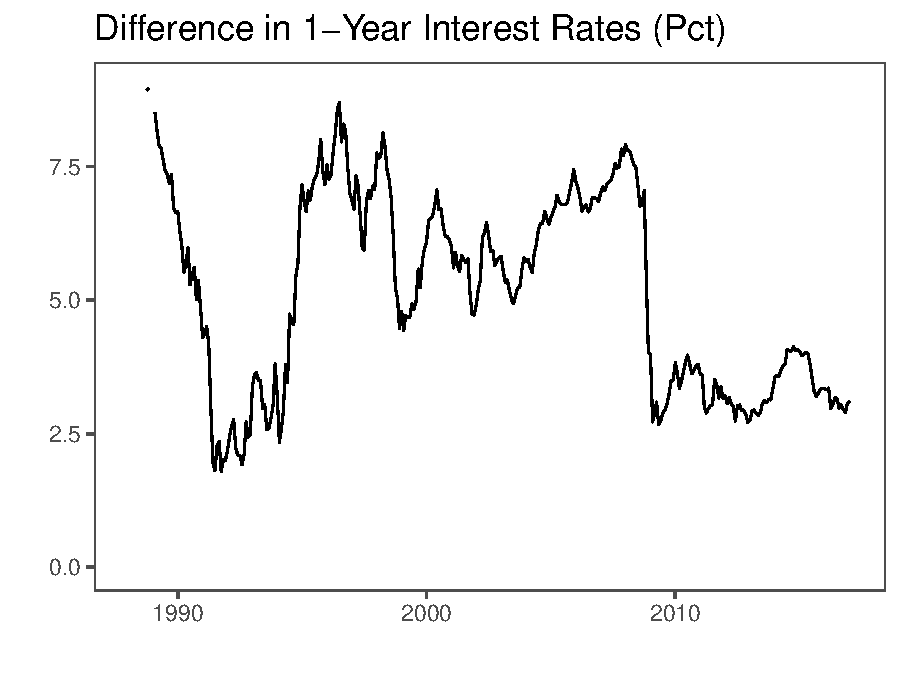
\includegraphics[width=\textwidth]{Exhibits/Figure_FP12M_DiffJPYNZD.pdf}
  \end{minipage}
  \begin{minipage}[htp]{0.49\textwidth}
  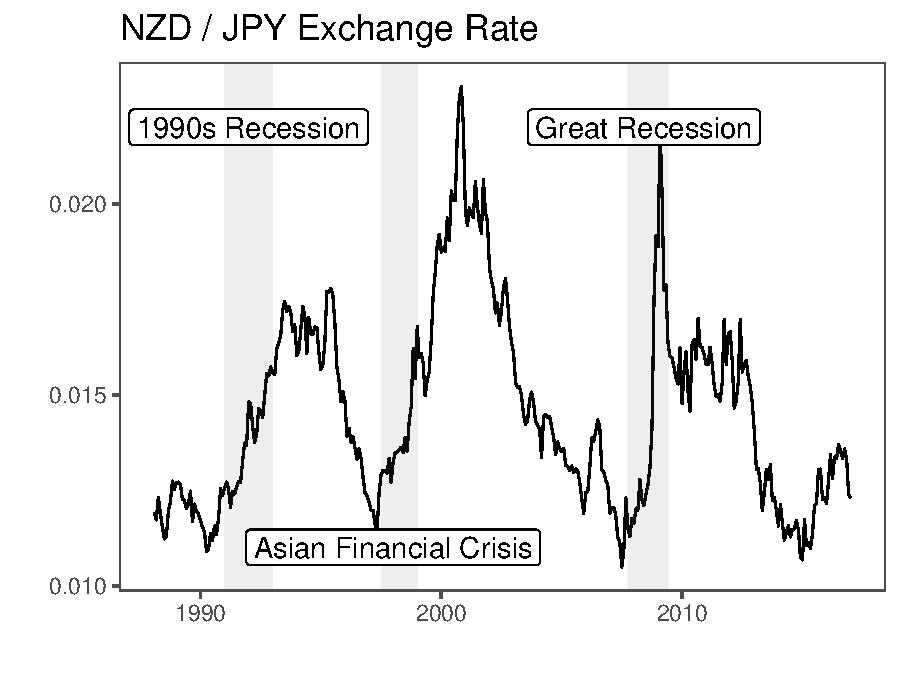
\includegraphics[width=\textwidth]{Exhibits/Figure_FX_JPYNZD.pdf}
  \end{minipage}
  
  \vspace{-1em}
  \begin{minipage}[htp]{\textwidth}
  \scriptsize
  \emph{Notes:} The left-hand panel plots the one-year risk-free interest rate in New Zealand dollars minus the one-year risk-free interest rate in Japanese yen. Risk-free rates are measured using each currency's one-year forward premia against the US dollar (USD). The right-hand panel plots the exchange rate of the New Zealand dollar (NZD) to Japanese yen (JPY) in units of dollars per yen. 
  \end{minipage}
\end{figure}
The left-hand panel of figure \ref{fig:fp} shows the difference in the risk-free interest rates of the New Zealand dollar and the Japanese yen as an example (we discuss below how one can measure such risk-free rates and compare them across countries). The figure shows the New Zealand dollar had a higher risk-free rate than the Japanese yen in \textit{every} month between January 1988 and December 2016. On average, this difference was about 5.26 percentage points (pp) on an annualized basis. When we adjust for movements in exchange rates over the period, the difference in returns on the two countries currencies is 5.10pp -- meaning a US investor who borrowed in Japanese yen and lent in New Zealand dollar made an average annualized excess return of 5.10pp over this period. (For comparison, the annualized excess return on US stocks was about 7.95pp during the same period.)

We now know such highly persistent differences in interest rates, similar to those between New Zealand and Japan, are common in the data, even among developed economies. These large differences in interest rates do not appear to be equalizing over time, and translate into large differences in returns investors can earn when investing in these currencies.

Why would $r^f$ differ permanently across countries? The emerging consensus in the literature is that the most likely explanation is currency risk premia -- the idea that some currencies are safer investments than others.

A useful way to think about this problem is to take the perspective of a retail investor in a third country, say, in Hong Kong. As is common in many countries, Hong Kong-based banks regularly offer savings accounts denominated in multiple currencies, so our fictitious investor might have the option to invest in yen at a deposit rate of 0.1\% or in New Zealand dollars at a rate of 3.0\%. How might she decide between these two options? Because both accounts are with the same bank, any likelihood of sovereign default is irrelevant. Similarly, our Hong Kong-based investor does not directly care about inflation in these two faraway countries. Instead, the only relevant factors for her choice between these two investments are the difference in interest rates and the stochastic behavior of the JPY-to-NZD exchange rate.

Because changes in exchange rates are largely unpredictable over short horizons, our investor should not expect either currency to depreciate over the coming year, leaving only one relevant consideration: covariance.\footnote{A regression of the log change in the JPY-to-NZD exchange rate on their interest-rate differential yields an R-squared of 0.00.} Which of the two currencies does our investor trust to retain value in a possible recession or crisis? Intuitively, she might think yen are a safer bet -- and she would be right.

Along with a number of other so-called ``safe-haven currencies,'' the yen tends to appreciate relative to the New Zealand dollar during large international recessions and crises. Figure \ref{fig:spot} shows some evidence of this pattern by plotting the NZD-to-JPY exchange rate in terms of dollars per yen (so that an increase in the exchange rate indicates yen appreciation). The shaded areas highlight three distinct periods of global economic turmoil: the early 1990s recession (1990 - 1993), the Asian financial crisis (1997 - 1998), and the Great Recession (2007 - 2009). In each of these periods, the yen appreciated markedly against the New Zealand dollar. If these appreciations during periods of economic turmoil are part of a broader pattern, investors should naturally consider the yen the safer currency -- and if yen are a safer store of value, accepting a lower deposit rate might make sense. That is, international investors might be willing to lend at lower rates in currencies they expect to retain value when times are bad.

As it turns out, this simple intuition has a lot of support in the data from international bond and derivatives markets. For example, a seminal paper by \citet{LustigVerdelhan2007} shows currencies with low interest rates tend to appreciate when US consumption growth is low, and depreciate when US consumption growth is high. That is, direct evidence shows currencies with low interest rates appreciate when times are bad for US consumers, making these currencies a safer store of value for US investors.

In addition to this empirical evidence, the theoretical work on currency risk has identified a number of theoretical reasons to expect the emergence of safe-haven currencies and long-lasting differences in interest rates. In a nutshell, persistent differences in countries' currency risk premia arise naturally in a wide range of international macro models. For example, \citet{Hassan2013} shows simply allowing for some economies to be larger than others within a conventional international real business cycle model is sufficient to generate long-term differences in interest rates between countries, because the currencies of larger countries tend to appreciate when worldwide output is low. That is, even within the most canonical, frictionless, international macro models, currency risk premia tend to arise naturally in equilibrium. Other authors have similarly pointed to the emergence of currency premia in models with intermediary capital constraints, trade costs, and differences in resource endowments, among others.

We survey the rapidly growing empirical and theoretical literature on currency risk premia in detail in sections \ref{sec_UIP} and \ref{sec_RP}. Because the initial focus of this literature was mainly on resolving asset pricing anomalies, many of its key papers tend to use technical finance language. For this reason, we attempt to keep this review as non-technical as possible, focusing primarily on the underlying economics.

A major difficulty this literature shares with a broader literature in asset pricing is that models with conventional preferences tend to produce risk premia that are quantitatively small. That is, although a number of papers have identified compelling reasons why, for example, the interest rate in Japan should be lower than that in New Zealand, most of these models suggest it should be lower by something on the order of 0.05pp rather than the 5.26pp we measure in the data. In this sense, the literature is running into a quantitative ``\textit{currency premium puzzle},'' which is in some ways analogous to the equity premium puzzle. Both puzzles fundamentally struggle with the prediction of models with standard preferences that risk premia should be small given the relatively small aggregate variation in consumption growth we measure in the data, though we also show the currency premium puzzle poses some unique challenges that have yet to be resolved. The development of quantitative models of currency risk and exchange rates is thus a major area for future research.

Although the literature on currency risk premia has proliferated in recent years, it has perhaps been less successful at making clear the relevance of its findings beyond the financial context, a gap we hope to partially fill with this article.

Perhaps the most immediate implication of currency premia for the real economy is for capital accumulation: If countries differ persistently in $r^f$, those with higher interest rates have a persistently higher cost of capital and thus, according to equation \ref{eq_one}, should produce with relatively less capital. Returning to our example from Figure \ref{fig:fp}, we find that, indeed, the capital-to-output ratio in New Zealand is 22\% lower than in Japan, suggesting the marginal product of capital is a lot higher in New Zealand than in Japan. More generally, countries with persistently higher interest rates appear to have higher marginal products of capital in the long run. This simple insight has direct implications for several strands of literature in macroeconomics, asset pricing, international finance, and monetary economics that have yet to be explored systematically.

The first is for the so-called Lucas Paradox \citep{Lucas1990}, which posits that over long periods of time, capital-to-output ratios do not appear to be equalizing across countries. In particular, not enough capital appears to be flowing to developing nations to equalize the marginal product of capital. If, indeed, some currencies are permanently riskier than others, currency risk is one possible factor preventing such equalization. Monetary and fiscal policies that reduce the perceived riskiness of a given currency could then also contribute to equalizing the marginal product of capital across countries. In addition, some of our own recent work suggests attracting investment by making one's currency a safer store of value for international investors may be a powerful motive determining the choice of a country's exchange rate regime \citep{HassanMertensZhang2020}.

A second, related, implication is for a large literature that focuses on assessing the efficiency of the allocation of capital across countries \citep{HallJones1997, CaselliFeyrer2007}. A basic assumption in this literature is that $r^f$ is equalized across countries, so that systematic deviations from this required rate can (partially) be attributed to inefficiencies. However, if fundamental (efficient) reasons exist for $r^f$ to differ due to differing currency (and country) risk characteristics, some of these calculations will have to be revisited -- possibly altering our assessment of how much of the discrepancy in income per capita across countries is to blame on inefficiencies.

Third, an active literature in international finance has studied the propensity of firms and governments to borrow in foreign currency \citep{cespedes2004balance, du2016sovereign}. If lending in a low-interest-rate currency is safer than lending in a high-interest-rate currency, the opposite is true for borrowing. That is, firms that borrow in dollar, yen, or other safe-haven currencies may be loading up on systematic risk -- a price they pay for enjoying lower rates. This systematic risk may then be a concern threatening the resiliency of firms' balance sheets and governments' solvency during major crises.

Finally, long-lasting differences in interest rates across countries may also change how we think about the sustainability of trade and current account deficits \citep{GourinchasRey2007} and the likelihood that different countries find themselves with nominal interest rates at the zero lower bound and differences in the efficacy of monetary policy.

The remainder of this article is structured as follows. Section \ref{sec_UIP} summarizes the empirical evidence that links currency risk to long-lasting differences in interest rates. Section \ref{sec_theory} reviews macroeconomic models of currency and country risk. Sections \ref{sec_capital} and \ref{sec_balancesheets} discuss implications for capital accumulation, exchange rate regimes, and currency risks on the balance sheets of firms and sovereigns.  Section \ref{sec_dynamics} discusses the link between time variation in currency risk and capital flows. Throughout, we highlight promising avenues for future research.


\section{Interest Rates and Currency Risk \label{sec_UIP}}

We begin by reviewing the major stylized facts on Uncovered Interest Parity (UIP) and related profitable trading strategies in currency markets. We then turn to the reduced-form evidence linking these anomalies to currency risk. 

\subsection{Failures of
  Uncovered Interest Parity and Profitable Currency Trades }

Early work on currency risk began as an attempt to understand three puzzling empirical facts in currency markets. The first, often referred to as the \textit{forward premium puzzle}, is that regressions of changes in the exchange rates on differences in interest rates yield a coefficient smaller than one. This fact suggests that, on average, high-interest-rate currencies do not depreciate enough to wipe out any differences in interest rates \citep{Bilson1981, Fama1984}. The second is that investors in the \textit{carry trade} appear to be making money by borrowing in currencies with low interest rates and lending in currencies with high interest rates. The third puzzling fact is that differences in interest rates and currency returns are highly persistent, so that the same countries tend to have high or low interest rates on a very long-term basis.

\begin{marginnote}[]
  \entry{Uncovered Interest Parity (UIP)}{For a given pair of currencies, the expected rate of depreciation should be equal to the interest differential: $$\mathbb{E}\Delta s^{f,h} = r^f_h-r^f_f.$$} 
  \entry{Forward Premium Puzzle}{A violation of UIP. Regressions of changes in the exchange rates on differences in interest rates yield a coefficient smaller than one.} 
  \entry{Carry Trade} {A violation of UIP. A profitable trading strategy that involves selling a portfolio of low-interest-rate currencies and buying a portfolio of high-interest-rate currencies.} 
\end{marginnote}

All three of these facts have in common that they describe different violations of UIP; that is, for a given pair of currencies $h$ and $f$, the expected rate of depreciation is usually not equal to the interest differential, $$\mathbb{E}\Delta s \neq r^f_h-r^f_f .$$ An extensive literature has documented these violations of UIP. \citet{Hodrick1987}, \citet{FrootThaler1990}, \citet{Engel1996}, \citet{Lewis2011}, and \citet{Engel2014} provide excellent surveys.\footnote{\cite{koijen2018carry} expand the notion of UIP to other asset classes and apply it to equities, bonds, and commodities.}

One difficulty for students of this literature is that it evolved simultaneously as an attempt to understand exchange rate dynamics (e.g., the forward premium puzzle) and asset pricing anomalies (e.g., the carry trade), and thus often alternates between regression-based and portfolio-methods that are not necessarily directly comparable to each other. We next give a brief overview using the unified approach by \citet{HassanMano2019}. This approach allows us to show the main empirical facts in a form where regressions map one for one into portfolios. However, it also forces us to abstract from many of the details uncovered in the two branches of the literature.

Following this approach, we implement the carry trade by forming a portfolio at the beginning of each month where we weight each currency $i$ by the difference between its risk-free rate, $r^f_{i, t}$ and the average risk-free rate of all currencies at the time, $\overline{r}^f_t$. That is, we go long currencies with high interest rates and short currencies with low interest rates such that we are long and short the same number of dollars. The return on this portfolio is
\begin{equation}
  \label{eq_carry}
  \textstyle\sum_{i}\left[ rx_{i, t+1}\left( r^f_{i, t}-\overline{r}^f_{t}\right) \right] ,
\end{equation}%
where $rx_{i, t+1} = r^f_{i, t} - r^f_{USD, t} + \Delta s_{t + 1}$ is the return to borrowing in USD and lending in foreign currency $i$ at between $t$ and $t+1$.

Implementing this strategy using one-month forward rates for 31 currencies between 1986 and 2010 yields an annualized mean return of 4.50\% with a Sharpe ratio of 0.54. For comparison, the Sharpe ratio of the US equity market during the same time period is 0.42. The carry trade is therefore a highly profitable trading strategy that rivals the equity premium and demands an explanation: Are carry traders being compensated for taking on risk? If so, what kind of risk are they taking?

We get the third fact mentioned above from decomposing these returns to the carry trade into a static and a dynamic component. Because interest rates do not change much over time, re-sorting the carry trade portfolio every month yields few benefits: on average, our carry trader would have still brought home 70\% of the same returns if she had used only three years of data on interest rates at the beginning of the sample to learn which currencies on average have high and low interest rates, sorted her portfolio once, and then never changed it afterwards.

\begin{textbox}[]\section{Measuring Risk-free Interest Rates and Currency Returns}
    In the US, we often regard T-Bills as risk free. However, even if we assume the US government cannot default, yields on the government debt of many countries are contaminated with the possibility of government default.

    For this reason, most of the recent literature constructs synthetic risk-free rates using currency forward contracts and applying covered interest parity (CIP) \citep{LustigRoussanovVerdelhan2011, DuSchreger2016}.\footnote{A forward contract is a rate at which a bank agrees to exchange one currency for another at a pre-specified date in the future.} To understand CIP, consider again our example of Japan and New Zealand, and suppose each country has a risk-free savings account. A Japanese investor with access to both accounts and to currency forward contracts then has two ways to make a risk-free investment in yen. First, she can simply save at the yen deposit rate. Alternatively, she can convert yen into New Zealand dollars at the spot exchange rate, invest the dollars at the local savings rate, and sign a forward contract to exchange her dollars back to yen at the end of her investment period. Both strategies are risk free because the spot and forward exchange rates are known today. Therefore, if no arbitrage occurs, the two strategies must yield the same return:
    \begin{equation}
    \underbrace{1 + r^f_{JPY}}_{\text{yen risk-free rate}}
    = \underbrace{
        (1 + r^f_{NZD}) \times \frac{S}{F}
    }_{\text{Implied yen risk-free rate}}.
    \label{eqn:CIP}
    \end{equation}
    Taking logs on both sides of this equation and showing $r_{JPY}-r_{NZD} = s - f$, the difference in risk-free interest rates must equal the difference between the (log) spot and forward exchange rates. This difference is known as the forward premium. As a result, we can reliably measure risk-free interest rate differentials from forward prices, even if a government's ability to repay its debts may be in question.\footnote{Prior to 2007, deviations from CIP have been on average close to zero. However, CIP deviations increased dramatically in magnitude for a number of countries during the Global Financial Crisis. This has led to a resurgence of interest in CIP deviations (see \citet{DuTepperVerdelhan2018}).} (For this reason, commercial providers of the carry trade also tend to implement it by buying and selling forward contracts, rather than by trading corporate or government bonds.)
\end{textbox}

In fact, \citet{HassanMano2019} show the incremental gain to re-sorting the carry trade portfolio every month is usually not statistically distinguishable from zero. To see how one could assess which variations in currency returns are statistically different from zero, note the carry trade return in equation \ref{eq_carry} is simply the covariance between currency returns at $t+1$ and interest differentials at time $t$. Thus, we can evaluate the expected return to the carry trade using a regression of the following form:
\begin{equation}
    rx_{i,t+1} - \overline{rx}_{t+1} 
    = \beta^{ct}\left( r^f_{it}-\overline{r}^f_{t}\right) +\epsilon_{i,t+1}^{ct},  \label{eq_ct}
\end{equation} 
where $\beta ^{ct}$ can be interpreted as the elasticity of expected currency returns with respect to interest rate differentials conditional on a time fixed effect. (For this interpretation, the right-hand-side variable in the regression, like the portfolio weights in equation (\ref{eq_carry}), must be known to investors at time $t$.) In our sample of 31 currencies, we estimate $\hat{\beta}^{ct}=0.57 (s.e.=0.19)$. Hence, within any time period, high-interest-rate currencies yield significantly higher returns than low-interest-rate currencies.

Moreover, this estimate also implies that for every dollar carry traders make on interest differentials, 1-0.57=0.43 dollars are wiped out by predictable depreciations. In other words, high-interest-rate currencies depreciate on average, but not by enough to eliminate the interest differential.

We should note some confusion in the literature on this point. In many older papers, authors show regressions of exchange rates on interest rate differentials with a country-specific intercept:
\begin{equation}
    \Delta s_{i,t+1} 
    = \alpha_i + \gamma \left(r^f_{i, t} - r^f_{US, t}\right) + \nu_{i, t+1},
\label{eq_fama} 
\end{equation}
and interpret the fact that the slope coefficient $\gamma$ is often negative as evidence that investors expect high-interest-rate currencies to \textit{appreciate} instead of depreciate. This finding has prompted a considerable theoretical literature trying to rationalize extremely volatile currency risk premia that are negatively correlated with predicted depreciations (the ``Fama conditions'', \citet{Backusetal2001}). However, this interpretation is incorrect, because a regression with currency fixed effects, such as equation \ref{eq_fama}, is not predictive -- investors at time $t$ do not know the fixed effect for each currency. \citet{HassanMano2019} show that once one corrects for this discrepancy between realized and predicted appreciations, one recovers results consistent withe the view that, on average, investors expect high-interest-rate currencies to depreciate, not appreciate.\footnote{This finding, of course, does not preclude the possibility that investors may expect or may have expected some high-interest-rate currencies to appreciate in specific historical circumstances. That is, the Fama conditions may be relevant in specific instances, but they do not describe the typical behavior of a typical currency in the post Bretton-Woods era.}

To summarize, the carry trade is highly profitable because highly persistent differences exist in risk-free interest rates across currencies that are only partially reversed by predictable depreciations. Currencies with higher interest rates yield higher returns on average to international investors than currencies with lower interest rates. Taken together, these three stylized facts form the empirical basis for the notion that long-lasting differences may exist in the risk characteristics of different currencies.

In addition to these major stylized facts, researchers have also documented a number of additional patterns in violations of UIP that have so far received relatively less attention from theorists. For example, \citet{ChinnMeredith2004} look at long-term bonds and find UIP tends to hold better at longer maturities. In other words, the currency of the high-interest-rate country tends to depreciate more over longer periods of time to negate some of the differences in interest rates. In related work, \citet{LustigStathopoulosVerdelhan2019} show the returns to currency carry trades also decrease with the maturity of the bonds. \citet{LRV2014} show another highly profitable trading strategy is the dollar carry trade: a trade in which investors buy non-US currencies whenever the average interest rate among advanced economies is higher than that of the US. 


\subsection{Interest Rate Differentials as Differences in Risk Premia \label{sec_RP}}

The conventional approach for attributing differences in returns to risk is to construct a \textit{risk factor} and check to what extent differences in covariance with this risk factor can account for differences in returns. Because knowing exactly what kind of risks investors may worry about may be difficult initially, a popular approach, going back to \cite{Fama1976}, is to construct this risk factor directly from asset returns. This method has been highly successful in studying stock returns, where researchers sort stocks based on some characteristic that is associated with a profitable trading strategy (e.g., the firm's market capitalization), and then divide them into a small number of portfolios based on the sort. The first portfolio typically contains stocks with the lowest values of the characteristic of interest (e.g., the smallest firms), and the last portfolio contains assets with the highest values (e.g., the largest firms). A risk factor is then constructed by taking the difference in returns between the first and last portfolio. Researchers determine a risk factor explains the differences in mean portfolio returns by running regressions of the returns to the remaining portfolios on the risk factor, and showing those portfolios with higher regression coefficients (``loadings'') on the risk factor also yield higher expected returns.\footnote{For example, \citet{FamaFrench1992} construct two risk factors by sorting US equities into portfolios based on market capitalization and book-to-market ratio, and show portfolios of stocks with greater exposure to these two risk factors obtain higher average returns.}

In a seminal paper, \citet{LustigRoussanovVerdelhan2011} applies these techniques to currencies and provide systematic evidence that the greater returns obtained from investing in high-interest-rate currencies result from greater risk exposure. For every month between November 1983 and December 2009, the authors sort currencies into six portfolios based on their risk-free rate differential relative to the US dollar. The first portfolio contains currencies with the lowest risk-free rates and the last portfolio contains currencies with the highest risk-free rates. The authors construct a \emph{carry trade risk factor} by taking the difference in the returns between the portfolio containing the highest-interest-rate currencies and the portfolio containing the lowest-interest-rate currencies.

\citet{LustigRoussanovVerdelhan2011} show that differential exposure to their carry trade risk factor accounts for cross-sectional variation in the expected returns from investing in different currencies. The authors regress the currency returns of their currency portfolios on the carry trade risk factor, and show the portfolios with higher-interest-rate currencies obtain a higher average return and also covary more positively with the risk factor. An increase in the loading on the carry trade risk factor from 0 to 1 is associated with a highly significant increase in excess returns of 5.5\% per year.

In this sense, \citet{LustigRoussanovVerdelhan2011} identify a common source of risk in currency markets, and show that exposure to this common source of risk accounts for cross-sectional differences in currency returns. However, the major drawback of this method is that it does not reveal the ultimate source of risk. In other words, we know exchange rates and currency returns co-move in a way that suggests common exposure to risk, but we do not know the economic forces that drive this co-movement.

Many researchers have therefore tried to identify relationships between currency returns and macro-financial variables to understand the sources of this currency risk. \citet{LustigVerdelhan2007} show that low-interest-rate currencies provide a hedge against US consumption growth risk. Low-interest-rate currencies systematically appreciate when US consumption growth is low, while high-interest-rate currencies tend to depreciate. US investors find this hedging property of low-interest-rate currencies useful, and, as a result, accept a lower rate of return on their investment.

Other studies highlight the resiliency of low-interest-rate currencies to periods of financial turmoil. \cite{lettau2014conditional} show that currencies with low interest rates tend to appreciate when US equity markets perform badly and, in this sense, have a lower ``downside beta,'' providing a hedge to stock market investors. They argue this variation in downside betas accounts for much of the returns to the carry trade. Similarly, both \citet{LustigRoussanovVerdelhan2011} and \citet{CampbellMedeirosViceira2010} argue that low-interest-rate currencies tend to appreciate in periods when equity markets are volatile, whereas high-interest-rate currencies tend to depreciate. Instead of using data from equity markets, \citet{Menkhoffetal2012} measure periods' financial market turmoil using an average realized exchange rate volatility. High-interest-rate currencies tend to depreciate in response to increases in the average realized exchange-rate volatility, whereas low-interest-rate currencies tend to appreciate. Thus, low-interest-rate currencies also provide a hedge against global exchange rate volatility. 

Another strand of the literature stresses the presence of crash risk as a possible driver of currency excess returns. \citet{Brunnermeieretal2009} study eight major currencies and show high-interest-rate currencies exhibit a greater chance of experiencing large devaluations (i.e., crash risk), whereas lower-interest-rate currencies do not. \citet{Jurek2014} formally assesses the share of carry trade returns explained by currency crash risk by constructing carry trades that are protected from crash risk. Specifically, \citet{Jurek2014} invests in a portfolio consisting of the carry trade as well as currency options that protect against large exchange-rate fluctuations (around 1.4 times the magnitude of the monthly standard deviation). He finds that buying protection from crash risk decreases the returns to the carry trade by about a third. Thus, the presence of crash risk explains about a third of the carry trade. \citet{Farhietal2015} propose a structural model of currency returns that are driven by the presence of crash risk. The authors calibrate the model using currency-options data and also find eliminating crash risk can reduce carry trade returns by a third.\footnote{These papers are also related to the literature on ``peso problems'' \citep{Lewis2011}, which occur when interest rates are high to compensate risk-neutral investors for an anticipated future currency devaluation.}

Ultimately, each of these papers highlights different ways in which high-interest-rate currencies may be riskier than low-interest-rate currencies. However, the common thread among these papers is that persistent differences in the returns to investing in different currencies reflect persistent differences in risk premia. Low-interest-rate currencies provide lower returns to investors because they are safer and tend to appreciate during periods of economic distress. Meanwhile, high-interest-rate currencies depreciate during periods of economic distress and must therefore reward investors with higher excess returns.



\section{Macroeconomic Models of Currency and Country Risk\label{sec_theory}}

Prompted by this reduced-form empirical evidence, the theoretical literature has identified several macroeconomic forces that may make a given currency safer or riskier from the perspective of global investors. Although which of these forces may be most important in practice has been the subject of an ongoing debate, many of these microfounded models share a common structure, which we can summarize using just a few key equations.

Consider a world economy in which international assets are priced by the marginal utility of an international investor, $m_T$, which will be our measure of ``good'' and ``bad'' times. Times are good when $m_T$ is low, and times are bad when it is high. In different models, $m_T$ may be the marginal utility of consumption of traded goods (the part of consumption that is shared internationally), the marginal utility of consumption of a key investor who intermediates between segmented international markets, or the capital constraint of such an intermediary. Households consume a country-specific final good, the price of which (accounted for in a common unit) depends on $m_T$ and a country-specific shock, $x^n$,
\begin{equation}
  p^{n} = a m_T + b x^{n}.  
  \label{eq_RF}
\end{equation}%
The country-specific shock interchangeably may stem from a country-specific supply, demand, or monetary shock; in other words, it is a stand-in for any factor that affects the price of consumption in one country more than in others. The higher $x^{n}$, the higher the price of domestic consumption relative to that in other countries. For simplicity, assume $m_{T} \sim N(0, \sigma^2_{m_{T}})$ and $x^{n} \sim N(0,\sigma^2_x) $ are normally distributed, not necessarily independent, shocks and $a$ and $b$ are positive constants.

The real exchange rate, $S^{f, h}$, between two countries $f$ and $h$ is the relative price of their respective consumption bundles. In logs,
\begin{equation}
  s^{f,h} 
  = p^f - p^h 
  = b(x^f - x^h),
\label{eq_RER}
\end{equation}
where lowercase variables denote logs and the second equality substitutes equation \ref{eq_RF}. Because of $x^{n}$, the relative price of consumption may differ between the two countries, allowing the real exchange rate to move. When the price of consumption in country $f$ increases, its consumption bundle appreciates relative to country $h$. In this sense, we can speak of ``currencies'' even without formally introducing money into the model.\footnote{For this reason, speaking of ``country risk'' rather than ``currency risk'' may be more appropriate. See the discussion in the text box labelled ``Currency vs.~Country Risk'' below. }

By definition, the risk-free bond in country $h$ pays $p^h$ with certainty, whereas that in country $f$ pays $p^f$ with certainty, so that each country's risk-free bond pays exactly one unit of that country's consumption bundle with certainty. However, because the real exchange rate may fluctuate, country $h$'s risk-free bond is not risk free from the perspective of households in country $f$, and vice versa. For this reason, one country's risk-free bond may be more expensive than the other country's risk-free bond. The risk-free rate of interest is the yield to maturity of the risk-free bond.  Hence, the country with the more expensive risk-free bond automatically must have the lower risk-free rate of interest. In this sense, any model with a variable real exchange rate as in equation \ref{eq_RER} may produce differences in risk-free interest rates across countries.

Different theories of such differences in interest rates apply elementary asset pricing to equation \ref{eq_RER} to show the log expected return to borrowing in country $h$ and to lending in country $f$ is
\begin{equation}
  r^{f} + \Delta \mathbb{E} s^{f,h} - r^{h} 
  = cov \left( m_{T}, p^{h}-p^{f}\right),
  \label{eq_UIP_RF}
\end{equation}%
where $r^{n}$ is the risk-free interest rate in country $n$.\footnote{$\Delta \mathbb{E} s^{f,h}$ is defined as the logarithm of the ratio of the countries' expected real price changes. See Appendix \ref{Appendix_ReducedFormResults} for a formal derivation.} Equation \ref{eq_UIP_RF} shows the currency that tends to appreciate when $m_T$ is high pays a lower expected return. Moreover, if $\Delta \mathbb{E} s^{f,h}\approx0$ (as is the case in the data), this currency also has a lower risk-free interest rate. In other words, a currency that appreciates in bad times (e.g., in times when consumption goods are expensive everywhere) provides a hedge against worldwide consumption risk and therefore pays lower returns in equilibrium.

\begin{textbox}[]
\section{Currency vs. Country Risk}
Although we follow the literature in referring to the spread in (\ref{eq_UIP_RF}) as stemming from ``currency risk,'' note that equations \ref{eq_RER} and \ref{eq_UIP_RF}, as well as virtually all models written on the subject, describe the stochastic behavior of the real, not the nominal, exchange rate. Fundamentally, what we mean by ``currency risk'' is therefore the risk that comes from country-specific shocks to a country's consumer price index. Different models may invoke various supply, demand, or monetary shocks for this purpose, but most models we discuss below actually do so without formally introducing money into the model. In this sense, speaking of ``country-specific risk'' or ``country risk'' is also accurate. 
\end{textbox}

Equations \ref{eq_RF} and \ref{eq_UIP_RF} are the main ingredients of risk-based models of differences in interest rates across countries. Different approaches identify various reasons why countries differ in the degree to which their price indices covary with $m_T$.

\paragraph*{Spillovers: Country Size and Trade Centrality}

Perhaps the most obvious reason for such differences in covariance to arise in the context of a microfounded model are differences in how important a given country is for the world economy. In particular, most models of exchange rate determination suggest any shock that raises the price of consumption in a larger economy also makes the part of consumption that is shared internationally more expensive. Thus, $m_T$ tends to rise more in response to a shock that raises the price of consumption in a larger country. As a result, their currencies retain value precisely when the marginal utility of international investors is high. The currencies of larger countries are therefore safer, have naturally lower interest rates, and pay lower returns to international investors \citep{Martin2012, Hassan2013}.

This result is easiest to see in a frictionless model with traded and non-traded goods. $m_T$ coincides with the marginal utility of traded consumption, which must be equalized across all countries in equilibrium, and $p^n$ coincides with the marginal utility of overall consumption in a given country $n$. Whatever country-specific supply, demand, or monetary shock raises a given country's $p^n$ then typically also prompts this country to import more traded goods. Whereas a small country's imports, by definition, have little or no effect on the world supply of traded goods, rising imports by a large country make traded goods relatively scarce in world markets, raising their price, and increasing $m_T$, so that
\begin{equation} 
    m_{T} = -c \sum_{n} \theta^n x^n,
    \label{eqn:lambdat2NP}
\end{equation}
where $c$ is a positive constant and $\theta^n$ is a measure of country $n$'s share of world GDP. It then follows that larger countries' consumption bundles tend to appreciate when $m_T$ is high. Comparing equation \ref{eqn:lambdat2NP} with equations \ref{eq_RER} and \ref{eq_UIP_RF} yields
\begin{equation}
  r^{f} + \Delta \mathbb{E} s^{f, h} - r^{h}
  =g\left(\theta^h - \theta^f\right) \sigma_x^2,
  \label{eq_FF_UIP}
\end{equation}
so that larger countries have lower interest rates, and their currencies are a safer store of value and pay lower returns on average.\footnote{If we allow for heterogeneity in the volatility of country-specific shocks $x^n$, the right-hand side of this formula generalizes to read $g(\theta^h
\sigma_{x,h}^2-\theta^f
\sigma_{x,f}^2),$ so that countries also have lower interest rates if they have more volatile country-specific shocks. \cite{to2019nontraded} show evidence of this pattern in the data.  }
  
Variations of this result in \citet{Hassan2013} also show that, by the same logic, firms producing non-traded (i.e., country-specific) goods in larger countries should have a lower cost of capital, and joining a currency union (an area that shares a common monetary shock) may lower interest rates in the participating countries.

More recent work by \citet{Richmond2019} highlights another force that may make a country's economy more important for the world economy: its trade centrality. Shocks to countries that are located near the center of the network of world trade, such as Singapore and the Netherlands, may have an outsized impact on the production of traded goods -- even if they are small. To arrive at this result, Richmond introduces multiple countries and non-traded goods into a model where traded goods are produced with intermediate inputs through a network of input-output linkages \citep{LongPlosser1983, Acemogluetal2012}. Within this framework, shocks that affect central countries spill over more to the rest of the world because these countries add a (small) amount of value to a large number of goods produced in the world. Shocks that raise the price of consumption in these central countries have an outsized effect on  $m_T$ because they are more disruptive to global supply chains. Therefore, the currencies of central countries are safer and pay lower interest rates than the currencies of peripheral countries.\footnote{\citet{LustigRichmond2020} provide further empirical support that currencies of countries that are geographically farther away from all other countries are riskier currencies.}   

This result relies on two key assumptions: First, shocks to the production of traded and non-traded goods are positively correlated within countries. In other words, the shocks that increase the price of domestic consumption must also raise the costs of its traded goods. Second, these shocks to production are more correlated across countries if two countries trade more with each other. (Both of these assumptions have broad empirical support.) \citet{Richmond2019} can then show $m_{T} = -c \sum_{n} \theta^n x^n- d\sum_{n} \nu^n x^n$, where $d$ is a positive constant and $\nu^n$ is a measure of the country's trade centrality.


\paragraph*{Differences in Stochastic Properties of Consumer Price Indices}

While both spillover-based approaches (size and centrality) put structure on which countries' shocks are more important for the marginal utility of international investors ($m_T$), another set of papers study innate differences in the stochastic properties of countries' consumer price indices ($p^n$).

\citet{FarhiGabaix2016} study a model where countries differ in their resilience to rare worldwide disasters. The non-traded goods of resilient countries increase in value whenever a disaster strikes, so that these resilient countries appreciate upon the disaster's impact -- making their currencies a safer store of value. Resilient countries therefore have lower interest rates, though how researchers should distinguish resilient from non-resilient countries in practice remains unclear.

\citet{Maggiori2013} argues the relatively low interest rates in the US may be explained if foreign exporters have relatively more trouble accessing trade credit in large financial crises. In his model, the stochastic discount factor depends on intermediary credit constraints, so that ``bad times'' occur when obtaining credit is difficult (i.e., in a financial crisis). If these credit constraints bind relatively more in countries that are less financially developed than the US, trade credit needed for shipping goods from the rest of the world to the US becomes relatively more expensive than trade credit for shipping goods from the US to the rest of the world in a crisis -- making the US consumption bundle relatively more expensive. He suggests this may be one reason why the US dollar tends to appreciate in extreme crisis periods, making the US dollar a safer store of value for international investors.\footnote{\citet{MalamudSchripf2020} also consider a model in which currency risk is determined by the risk-bearing capacity of country-specific financial intermediaries. Financial intermediaries with more risk-bearing capacity, are more able to ensure their households against economic downturns. As a result, their currencies are more valuable and tend to appreciate during times.}

\citet{Readyetal2013} note that a number of ``commodity countries,'' such as Norway and Australia, largely export basic commodities, such as coal, oil, and iron ore, but rely much more on imports of finished goods than ``producer countries,'' such as Japan and Germany, which export these goods. In their model, worldwide shipping capacity can only adjust slowly over time. In a boom, when output of traded goods is high, more commodities must be shipped from the commodity countries to the producer countries, and more finished goods in the opposite direction. This increased demand for shipping drives up trade costs disproportionately more in the commodity countries because, in effect, any finished goods they consume must travel farther. Therefore, the price of consumption in commodity countries increases in a boom (when $m_T$ is low) and decreases in a downturn, relative to the price of consumption in producer countries. It follows that, in effect, commodity countries appreciate in ``good times'' and depreciate in ``bad times.'' With quadratic shipping costs, we have
\begin{equation*}
  p^{\text{Commodity Country}}-p^{\text{Producer Country}}\sim\left(\frac{\text{Finished goods shipped}}{\text{Shipping Capacity}}\right)^2.
\end{equation*}
An additional implication of this model is that the real exchange rates of commodity countries are positively correlated with worldwide commodity prices. 

\citet{Powers2015} derives similar results without appealing to stochastic trade costs, but instead argues commodity booms drive up wages in commodity countries, so that local non-traded goods become more expensive through a Balassa-Samuleson-type labor-cost effect. The consumption bundles of commodity exporters therefore tend to appreciate in worldwide booms and depreciate in worldwide busts, making their currencies riskier than those of non-commodity-exporting countries.

Aside from commodity-producing countries, \citet{Wiriadinata2020} points out that countries that have a large amount of outstanding dollar-denominated external debt tend to depreciate whenever the dollar appreciates, and have high interest rates and currency returns. She rationalizes this pattern with the wealth effect: when the US dollar appreciates, the real value of dollar-denominated debt increases, effectively making countries that borrow in dollars poorer. This negative wealth shock in turn reduces domestic demand, lowering the relative price of domestic non-traded goods, and thus depreciating the currencies of countries that borrow heavily in dollars.

\paragraph*{Portfolio Balance Models} Another ``portfolio balance'' approach to understanding currency risk directly models the capital constraints of financial intermediaries engaged in currency trading. \citet{GabaixMaggiori2015} consider a world in which a financier with limited risk-bearing capacity must absorb any imbalances in the supply and demand for currencies across countries. The financier is willing to do so only if she earns positive expected returns on the currencies she holds in her portfolio, so that any currency that is in excess supply must earn higher expected returns in equilibrium.  \citet{GabaixMaggiori2015} suggest that, in practice, financiers are holding assets of net-debtor countries. As a result, investing in net-debtor countries' currencies should obtain positive excess returns. \citet{DellaCorteetal2016} provide systematic evidence for this hypothesis in the data, and furthermore show the currencies of net-debtor countries systematically depreciate in times of financial turmoil. 

In a recent paper, \citet{LiaoZhang2020} study a portfolio balance model in which the stochastic properties of currencies are determined by investor hedging demands. When investors in a net-debtor country trade with financial intermediaries for the purposes of hedging their net foreign asset position, the financial intermediaries must sell the net debtor country's currency, which leads to currency depreciation. In practice, investors tend to increase their hedging demands during periods of financial turmoil. As a result, the currencies of net-debtor countries tend to depreciate during periods of financial turmoil and are thus systematically riskier.
 
 
\begin{textbox}[h]
\section{Foreign Asset Portfolios and the Reserve Currency Paradox} Whereas we have focused our discussion on interest differentials and violations of UIP, most models make additional predictions about the returns on other assets (e.g., stocks in the traded and non-traded sector), the composition of equilibrium portfolios, and the co-movement of consumption across countries. One common prediction in models where households share risk across countries is that countries with low interest rates should also be net importers of insurance from the rest of the world. 

This result is easiest to see in equation (\ref{eq_BFT}): countries with lower interest rates have more volatile marginal utility, so they need and want relatively more insurance. That is, the same forces that make a given country's currency relatively safe will also tend to make this country a net importer of insurance from the world market. 

Although the link between country risk and net foreign asset portfolios has not been systematically studied in the data, this prediction appears at odds with the US data, which is generally seen as having both a low interest rate and being a net exporter of insurance to the rest of the world (US investors tend to hold equity abroad, whereas foreign investors largely hold US safe assets, such as T-Bills, \citep{GourinchasRey2007,GourinchasGovillotRey2017}). \cite{Maggiori2013} calls this puzzling pattern in the US data the ``reserve currency paradox.'' Aside from resolving this puzzle for the US, future research should also explore whether the same puzzling pattern extends to the portfolio holdings of other low-interest-rate countries. 
\end{textbox}


\subsection{Reduced-Form Evidence}

Although many of the theoretical papers surveyed above provide detailed evidence on each of the particular channels making a given currency safer or riskier from the perspective of world investors, the literature currently lacks a comprehensive evaluation of their relative importance. As a first step in this direction, Table \ref{table:rx_char} shows a set of regressions of currency returns for 31 currencies between 1998 and 2016 on variables that, according to various theories, should be associated with lower interest rates and returns. 
\begin{table}[htp]
\begin{center}
\caption{Currency excess returns and characteristics}
\label{table:rx_char}
\vspace{1em}
\begin{tabular}{l c c c c c }
\hline
\hline
 & (1) & (2) & (3) & (4) & (5) \\
\hline
GDP Share               & $-0.50^{**}$ &             &               & $-1.27^{***}$ & $-1.51^{***}$ \\
                        & $(0.25)$     &             &               & $(0.34)$      & $(0.39)$      \\
Trade Centrality              &              & $-0.41^{*}$ &               &               & $0.43$        \\
                        &              & $(0.22)$    &               &               & $(0.26)$      \\
NIIP / GDP              &              &             & $-0.84^{***}$ &               & $-0.85^{***}$ \\
                        &              &             & $(0.25)$      &               & $(0.23)$      \\
FX Allowed Deviation         &              &             &               & $0.20^{***}$  & $0.15^{*}$    \\
                        &              &             &               & $(0.05)$      & $(0.08)$      \\
\hline
Fixed Effects & Time & Time & Time & Time & Time \\
Num. obs.     & 7,517        & 7,517     & 6,177          & 6,488          & 5,186          \\
R$^2$         & 0.27        & 0.27     & 0.32          & 0.28          & 0.33          \\
\hline
\hline
\end{tabular}
\end{center}
\begin{minipage}[htp!]{\textwidth}
\scriptsize
\emph{Notes:} This table presents regressions of currency excess returns on currency-area characteristics. GDP Share is a currency area's share of world GDP. Centrality is a currency area's trade centrality taken from \citet{Richmond2019}. NIIP / GDP is a currency area's net international investment position as a share of GDP \citep{DellaCorteetal2016}. FX Allowed Deviation captures each currency's maximum allowable annual exchange rate deviation relative to its target currency according to \citet{ilzetzki2018exchange}. Standard errors are clustered by currency region. $^{***}p<0.01$, $^{**}p<0.05$, $^*p<0.1$
\end{minipage}
\end{table}

The first three columns show a one standard deviation increase in a country's size (GDP share), trade centrality, and net foreign asset position are associated with 0.5pp, 0.4pp, and 0.8pp decreases in the returns on the country's currency, respectively. In addition, column 4 shows that currencies that are stabilized relative to the US dollar or the euro (a lower FX Allowed Deviation) also have significantly lower returns. (We discuss this finding in section \ref{sec_regimes} below.) When we combine all four variables in column 5, trade centrality loses significance.

Although these results are suggestive, they are also inadequate. Because interest differentials are highly persistent, all of these regressions rely primarily on cross-sectional variation for identification.  With fewer than 40 currencies for which we have reliable data, our statistical power for disentangling the effect of multiple variables is limited. Moreover, these regressions have no way to account for the ease with which each of the candidate mechanisms can account for the various auxiliary predictions of each of these models. A key challenge to the literature is thus to develop and compare quantitative models of currency risk.


\subsection{Quantitative Models and the Currency Premium Puzzle \label{section:cpp}}

Quantitative work on currency risk is perhaps surprisingly under-developed and a major area for future research. Only one or two papers even attempt to match differences in interest rates as large as those shown in Figure 1, and perhaps even more surprisingly, not a single paper speaks to the correspondingly large differences in capital-to-output ratios between countries we see in the data. Two major reasons explain this lack of progress.

The first is a little recognized asset pricing puzzle -- we call it the \textit{currency premium puzzle}. The essence of this puzzle is that the surprisingly large currency risk premia pose a fundamentally different challenge to theorists than the equity premium puzzle. To see this challenge, recall that much of contemporary asset pricing theory was developed to reconcile a large equity premium with the fact that aggregate consumption data are relatively smooth. To rationalize a mean excess return of stocks over bonds of 8\% with a standard deviation of 16\%, as we see in US equity markets, \citet{HansenJagannathan1991} show the stochastic discount factor (the marginal utility of overall consumption in most macroeconomic models) $m$ must have a standard deviation of at least 0.5, whereas the standard deviation of annual aggregate US consumption growth is an order of magnitude smaller (about 0.03).  

To see how this challenge differs from the currency premium puzzle, we can rewrite equation \ref{eq_UIP_RF} to read as follows: 
\begin{equation}\label{eq_BFT}
  r^{f} + \Delta \mathbb{E} s^{f,h} - r^{h} 
  =-\frac{1}{2}\left(var(m^f)-var(m^h)\right),
\end{equation} 
where $var(m^n)$ denotes the variance of the stochastic discount factor measured in units of the consumption bundle specific to country $n$.\footnote{This formulation is originally due to \cite{Backusetal2001}. However, the traditional reading of this equation, prior to the work by \cite{LustigRoussanovVerdelhan2011} and \cite{HassanMano2019}, has not focused on rationalizing persistent differences in currency returns, but rather the (as we argue overstated) idea that currencies tend to appreciate when they have unusually high interest rates -- the Fama conditions.} Thus, if we assume the standard deviation of $m^{Japan}$ is 0.5 (at the Hansen and Jagannathan bound), the standard deviation of $m^{New Zealand}$ would have to be 0.4 -- or 20\% lower -- to justify the observed differences in interest rates. That is, to solve the currency premium puzzle, a quantitative model not only has to make marginal utility much more volatile than aggregate consumption, but also has to amplify differences in the volatility of marginal utility across countries to the point that they are multiple times larger than the standard deviation of aggregate consumption growth. Although many modern finance models are equipped to do the former, whether they can be re-tooled to also achieve the latter is unclear. 

An added difficulty for these models is that, empirically, the majority of differences in currency returns come from differences in interest rates, and not from predictable depreciations. Technically, matching this empirical fact requires generating large differences across countries in $var(m^n)$ without generating large differences in conditional expectations $E_t(m^n)$. 

The second major challenge to microfounded quantitative models of currency returns is that all of these microfoundations of course rely on introducing substantial heterogeneity in various dimensions (country size, trade centrality, commodity endowments, etc.). This requirement contrasts with traditional solution methods in finance and macroeconomics, where the former tend to be designed for closed economies, whereas the latter either target two symmetric countries or one small country that is measure zero in the world economy. Introducing a large, but finite, number of heterogeneous agents that make decisions affecting the equilibrium allocation within a dynamic framework while solving for risk premia is thus a challenge for which relatively few tools exist. 


\citet{colacito2018currency} make an important first step in this direction by adding multiple countries that differ in their exposure to a global long-run endowment shock to a quantitative model with long-run risk and recursive preferences. They measure these different exposures in the data for the G7 economies and argue these exposures can be thought of as a reduced-form representation of the various fundamental drivers of country risk surveyed above, which all ultimately suggest some countries are more affected by global downturns than others. \citet{colacito2018currency} then show a reasonable calibration of their model can replicate large differences in currency returns across countries that align nicely with the returns on high and low-interest-rate portfolios in \cite{LustigRoussanovVerdelhan2011}.\footnote{ Interestingly, because the model produces a tight link between interest rates and the portfolios held by each country (see our discussion of the reserve currency paradox above), this sorting on interest rates closely corresponds to a sorting of currencies on the country's net foreign asset position as suggested by \citet{DellaCorteetal2016}.} 
An added benefit of their framework is that the combination of long-run risk with recursive preferences also resolves the forward premium puzzle and matches a number of other facts about the dynamics of exchange rates and interest rates, as the authors show in their earlier work \citep{ColacitoCroce2011}. 

However, one difficulty the authors were unable to resolve is that the majority of the carry trade returns in their model stem from predicted depreciations, whereas interest rate differentials account for only about one third of these returns quantitatively. This issue, and tying the reduced-form exposures to global risk to their economic origins, thus remain major areas for future research.


\section{Currency Risk and the Allocation of Capital across Countries\label{sec_capital}}

Equation \ref{eq_one} suggests firms in countries with high-interest-rate currencies should accumulate less capital and operate at a higher marginal product of capital than those in low-interest-rate countries. Indeed, solving for differences in capital intensity across countries within models of currency risk yields this result. For example, \citet{HassanMertensZhang2015} find that in a model with differences in country size,  
\begin{equation}
    k^f - k^h = d
    \left(r^h - \Delta \mathbb{E} s^{f, h} - r^f \right),
\end{equation}
where $d$ is a positive constant and $k^n$ denotes capital intensity in country $n$. That is, the class of models surveyed above generally predicts long-lasting violations of UIP should pass through to capital accumulation, so that currency risk directly affects the allocation of capital across countries and firms.

This theoretical result can be thought of in two equivalent ways. First, firms based in countries with safer currencies should have a lower cost of capital, which increases their value in world markets and prompts them to invest more.\footnote{This lower cost of capital generally applies to all firms that produce country-specific goods (whose value naturally co-moves with the exchange rate), but not to firms that produce a homogeneous traded good.} Second, from a risk-sharing perspective, accumulating more capital in countries that are large or in other ways ``systemic'' is efficient, because shocks that affect consumption in these countries tend to spill over more and affect allocations globally. A social planner thus has a precautionary motive to allocate more capital to the countries that have the largest spillovers. That is, one need not appeal to prices to understand the effect of currency risk on capital accumulation.

%Using this result, \citet{HassanMertensZhang2015} estimate a dynamic model with heteogeneous currency risk and endogenous capital accumulation and find that variation in currency risk across seven industrialized countries explains about two thirds of the variation in capital to output ratios between them. However, the magnitude of the differences in capital accumulation fall short of those observed in the data.

Figure \ref{fig:ky_rx} shows a strong negative relationship between capital accumulation and currency excess returns for our sample of 31 countries. The slope shown suggests a 1pp increase in the returns on a given currency is associated with a 0.26 level decrease in the issuing country's capital-to-output ratio (corresponding to a decrease of 0.24 of one standard deviation). Altogether, variation in currency premia accounts for slightly less than a quarter of the variation in capital-to-output ratios across countries. The corresponding regression of $K/Y$ on interest rate differentials similarly shows a negative relationship (coef = -0.10). The aggregate data thus show clear evidence consistent with a link between currency risk premia and capital intensity. 
\begin{figure}[htp]
    \centering
    \caption{Capital intensity and currency excess returns}
    \label{fig:ky_rx}
    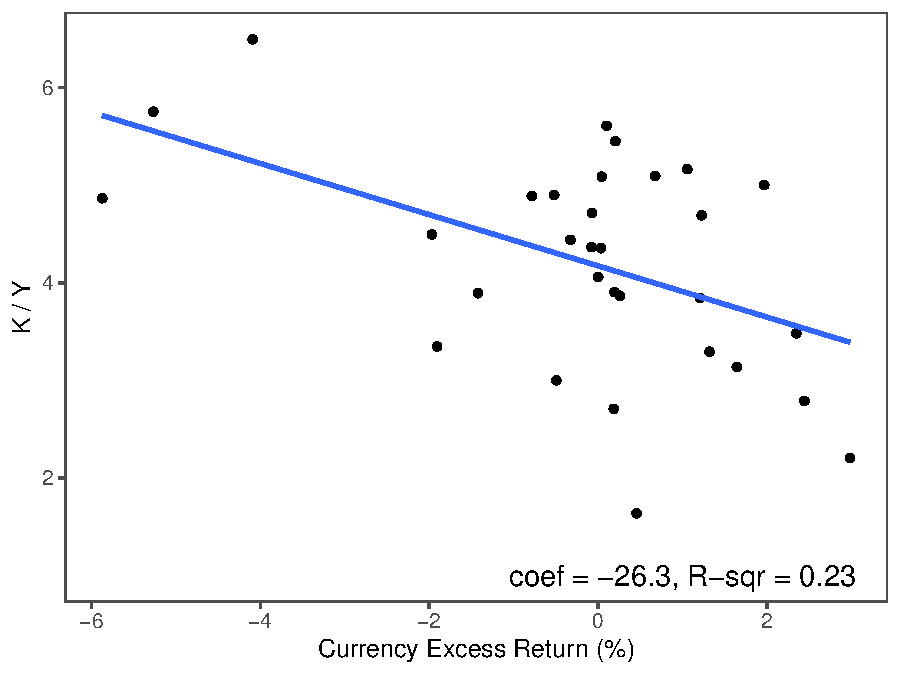
\includegraphics[width=0.7\linewidth]{Exhibits/Figure_KY_RX.pdf}
    \begin{minipage}[htp]{\textwidth}
    \scriptsize 
    \emph{Notes:} This figure shows the relationship between average currency excess returns and average capital-to-output ratios across currency regions. The sample comprises the same set of 31 currencies from 1988 to 2016 used to produce Table 1. The line of best fit has a slope of -0.26 (s.e. = 0.01). R-sqr = 0.23. The corresponding coefficient on a regression of capital-to-output ratios on interest rate differentials is -0.10.
    \end{minipage}
\end{figure}

Pushing beyond the aggregate data, \citet{Richers2020} shows direct evidence of an effect of currency premia on the cost of capital at the firm level: using data from the primary issuance of 100,000 corporate bonds of non-financial firms in 98 countries, he shows that differences in risk-free interest rates pass through almost one for one to firms' cost of borrowing. That is, firms borrowing in low-interest-rate currencies have cheaper access to credit than their counterparts that borrow in high-interest-rate currencies. These differences in bond-level yields cannot be explained with observable characteristics of firms issuing in different currencies (e.g., their credit rating, accounting ratios, etc.), and even exist within firms that issue in multiple currencies within the same month. That is, the same firm issuing in Japanese yen and New Zealand dollars in the same month pays a several percentage point higher yield to maturity on the latter bond than the former bond.

Consistent with these patterns, \citet{Richers2020} also shows that firms that are headquartered in countries with higher interest rates produce more output per unit of capital installed, again suggesting these firms indeed operate at a higher marginal product of capital.

\citet{DavidHenriksenSimonovska2014} add further evidence in favor of a risk-based interpretation of these patterns. They show that although the returns to capital investment are higher in emerging market economies, they are also more correlated with the US stock market. This pattern suggests emerging market economies are more exposed to systematic risk, which the authors interpret as long-run growth risk. Thus, capital investment in emerging markets should pay higher returns to compensate investors for this risk exposure. The authors go on to calibrate a model with recursive utility where countries are exposed to long-run growth risk according to their empirical correlation with the US stock market. Their model is able to quantitatively account for a significant portion of the variation in capital accumulation across countries.

This link between a country's risk characteristics and capital accumulation poses challenges and opportunities for several ongoing debates in the macroeconomics literature that have yet to be explored systematically and may prove fertile ground for future research. We outline each of these potential applications briefly below.

\subsection{The Lucas Paradox}

Perhaps the most important conclusion from research on currency risk to date is that differences in interest rates between countries are tied to fundamental forces determining their risk characteristics and are therefore here to stay for the long term. This view is at odds with a long history of thought in macroeconomics going back to \cite{solow1956contribution} that has traditionally viewed differences in the marginal product of capital across countries as transitory. In particular, a large literature following \citet{Lucas1990} has been trying to reconcile large differences in the measured marginal product of capital across countries with the fact that not enough capital seems to be flowing across countries to equalize these marginal products, particularly from developed to emerging economies (the ``Lucas Paradox''). 

The existing literature has debated various potential resolutions to the Lucas paradox and the associated lack in convergence in GDP per capita across countries. These resolutions include accounting for heterogeneity in the protection of property rights \citep{HallJones1997}, in taxation rates \citep{Jorgenson1996}, in depreciation rates, in the capital share of output \citep{Neiman2014}, in distortions in the allocation of resources \citep{HsiehKlenow2009}, and in the role of natural resources in production \citep{CaselliFeyrer2007, Monge-Naranjoetal2019}.  The common assumption in this literature, however, is that in the absence of these frictions, interest rates, and the marginal product of capital should eventually equalize across countries.

To our knowledge, neither the role of persistent differences in risk free interest rates nor the role of currency risk have been systematically evaluated relative to this literature. In other words, one reason why we observe persistent differences in the marginal product of capital and see a lack of convergence in GDP per capita across countries may simply be persistent differences in currency and country risk. Thus, one avenue for future research is to test whether differences in currency risk can quantitatively account for the observed differences in capital-output ratios. If accounting for differences in currency risk is indeed useful for understanding the Lucas paradox, then the task of understanding the ultimate sources of currency risk still remains, as discussed in section \ref{sec_theory}. However, these ultimate sources of currency risk must now also account for differences in capital accumulation across countries. 

\subsection{Currency Risk and Exchange Rate Regimes\label{sec_regimes}}

In addition to potentially shedding light on these long-standing puzzles about the lack of convergence in MPK across countries, a recent paper by \citet{HassanMertensZhang2020} argues the link between the stochastic properties of a country's real exchange rate and the level of capital accumulation also provides a new way of thinking about the costs and benefits of adopting different exchange rate regimes. The authors note the pervasive practice among small and medium-sized economies to stabilize their exchange rate relative to the US dollar or the euro \citep{ilzetzki2018exchange} may be thought of as an attempt to make their currencies (and by extension their economies) a safer investment from the perspective of world investors. 

In their model, countries again differ in size, and the domestic prices of traded goods are sticky in terms of the domestic currency, so that each country's central bank has some control of its country's real exchange rate. When a small country stabilizes its exchange rate relative to a larger target country, its real exchange rate inherits the stochastic properties of that larger target currency and thus becomes safer from the perspective of world investors. A safer currency in turns comes with a lower domestic risk-free rate, higher domestic capital accumulation, and higher wages. That is, managing a country's exchange rate risk becomes a means of attracting international investment and raising the world-market value of domestic firms. In the absence of policy coordination, small countries then optimally choose to stabilize their exchange rates relative to the currency of the largest economy in the world, which endogenously emerges as the world's anchor currency. Larger economies instead optimally choose to float their exchange rates, because currency interventions by larger countries are endogenously more expensive to maintain than those by smaller countries. The model therefore predicts an equilibrium pattern of exchange rate arrangements that fits the data, where almost all stabilizations target the same anchor currency (the USD), small countries below a certain size stabilize, intermediate-sized countries maintain weaker stabilizations, and only the largest economies in the world float their currencies. 

\section{Currency Risk, Macroprudential Regulation, and Monetary Policy \label{sec_balancesheets}}

Beyond its consequences for the allocation of capital across countries, the study of currency risk also potentially poses questions relating to monetary policy, and macroprudential regulation.

First, a large literature on the ``currency mismatch'' highlights that borrowing in foreign currencies exposes the borrower to the risk of default in an event of an appreciation of the foreign currency \citep[e.g]{EichengreenHausmann1999,cespedes2004balance}. Indeed, although the propensity of governments to issue debt in a foreign currency has decreased over time, firms often choose to issue debt in low-interest-rate currencies -- particularly those firms that are based in emerging markets \citep{DuSchreger2016}. Our discussion of currency risk adds an important wrinkle to this debate: all currency mismatch is not created equal. Instead, if currencies such as the dollar and the euro have low interest rates because they appreciate in times of economic distress, firms that borrow in these currencies are effectively selling insurance against that distress, because the real value of their liabilities increases in those states of the world. In other words, borrowing in low-interest-rate currencies is not a free lunch, but instead exposes the borrower to systematic risk. This link between borrowing in low-interest-rate currencies and systematic risk may provide a rationale for regulatory intervention that limits the amount of foreign-denominated debt certain firms can issue.

Recent evidence by \citet{liao2020}, \citet{Richers2020}, and \citet{SalomaoVarela2019} shows that denominating part of their debt in low-interest-rate currencies allows firms to lower their overall cost of capital, invest more, and lower their mean return on assets. Moreover, \citep{KalemliOzcanetal2019} shows firms can be further exposed to the currency risk through foreign currency loans from domestic banks. As credit conditions vary over the business cycle, firms shift the currency denomination their borrowing toward the low-interest-rate currency.\footnote{A related literature has highlighted the consequences of the currency denomination of corporate debt for the risk of sovereign default \citep{DuSchreger2016, OttonelloPerez2019}.} In this sense, we have a growing body of evidence that shows the upside of issuing debt in low-interest-rate currencies: a lower cost of capital. 

By contrast, very little is known about Which firms, households, and governments can and should take on this systematic risk. A number of recent papers suggest interesting interactions between currency risk, exchange rate policy, and regulation. \citet{Bocola2019} study one such example, where savers prefer to denominate deposits in dollars rather than the domestic currency, because they expect the dollar to retain value and appreciate during recessions. Domestic issuers meet this demand by denominating their debt in dollars, creating a currency mismatch. Interestingly, the authors show ex-post bailouts to borrowers can be an attractive policy alleviating the country's susceptibility to crises. \citet{SalomaoVarela2019} develop a structural model of the currency denomination of debt. In their model, productive firms with a high marginal product of capital optimally take on currency risk. Moreover, the authors also highlight interesting interactions between the local government's choice of exchange rate regime and the allocation of currency exposure across firms. \cite{keller2019capital} studies foreign currency borrowing by corporations in Peru and shows capital controls meant to reduce such foreign currency exposure may actually end up increasing it. \citet{du2020sovereign} instead analyze a model in which risk averse lenders demand a risk premium for lending in the domestic currency, because the monetary authority would like to inflate away domestic currency debt during economic downturns. Thus, governments without the ability to commit to a low inflation target optimally issue foreign currency debt to avoid paying an inflation risk premium on domestic currency debt. 


A second, potentially important implication of long-lasting differences in risk-free interest rates is that countries with lower risk-free rates may be more likely to find themselves at the zero lower bound on nominal interest rates. Although whether the Federal Reserve should raise its inflation target in times of ultra-low rates has been debated \citep{coibion2012optimal,holston2017measuring,mertens2018expect}, we are unaware of any work on how inflation targets or other aspects of monetary policy should vary across countries with ordinarily high and low risk-free rates. 

\section{The Dynamics of Currency Risk\label{sec_dynamics}}

Up to this point, we have focused our discussion on the cross-sectional variation in currency risk, which has also been the focus of the most recent literature. A natural extension of this discussion is to understand the variation in currency and country risk over time, and in particular the role such fluctuations may play in driving variation in capital flows across borders.

As stated in section \ref{sec_UIP}, much of the early work on currency risk began as an attempt to understand the forward premium puzzle --- the finding that, on average, high-interest-rate currencies do not depreciate enough to wipe out any differences in interest rates. In addition, many studies have highlighted an apparent disconnect between macroeconomic variables and variation in exchange rates \citep{MeeseRogoff1983}, and exchange rates appear surprisingly volatile compared with aggregate consumption growth \citep{BackusSmith1993}. In response to these empirical facts, a large theoretical literature has argued time variation in currency risk premia may be able to jointly rationalize these facts \citep{Fama1984,Backusetal2001}.

One strategy for introducing large amounts of time variation in currency risk premia involves using more complicated investor preferences from the asset-pricing literature that have helped resolve other asset-pricing anomalies. \citet{Verdelhan2010} proposes a model in which representative investors of each country exhibit preferences for an exogenously specified ``habit'' level of consumption. As a country's consumption approaches its habit level, the domestic investor becomes more risk averse. This increase in risk-aversion lowers the domestic interest rate while inducing a predictable depreciation. This additional force moving exchange rates then rationalizes the apparent exchange rate disconnect we see in the data. In the extreme, this mechanism can also rationalize a situation where investors expect currencies that have unusually high interest rates to appreciate instead of depreciate (the ``Fama conditions'').  Building on this intuition, \citet{Heyerdahl-Larsen2011} shows that adding ``deep habits'' -- habits for specific goods within the consumption basket -- allows the model to match the term structure of bond yields as well the dynamics of exchange rates. Moreover, \citet{Stathopoulos2017} shows one can also rationalize the low volatility of real exchange rates and the disconnect between exchange rates and consumption by adding consumption home bias (in addition to habit preferences). 

An alternative assumption is to endow investors with \cite{EpsteinZin1989} utility functions and allow for long-run risks. Within these models, shocks to expected long-term consumption growth strongly influence exchange rates today -- again producing an apparent disconnect with contemporaneous consumption growth and other macroeconomic variables. \citet{ColacitoCroce2011} show a model with highly correlated long-term growth shocks can produce a low correlation in consumption across countries along with a realistic volatility of exchange rates. \citet{BansalShaliastovich2012} and \citet{ColacitoCroce2013} further show long-run news shocks in combination with a high intertemporal elasticity of substitution also produce the kind of co-movement of interest rates and currency risk premia required to explain the forward-premium puzzle. 

Another strategy for introducing time variation in currency risk premia is to assume time variation in the probability of rare disasters. \citet{FarhiGabaix2016} show time-varying disaster risk can produce realistic time-varying currency risk premia. In contemporaneous work, \citet{GourioSiemerVerdelhan2011} study a quantitative model with time-varying rare disasters and show the presence of rare disasters generates volatile exchange rates, large currency risk premia, and an apparent disconnect between exchange rates and macroeconomic fundamentals that is consistent with the data.

These papers all have in common that they study the interaction of two ex-ante symmetric countries, and abstract almost entirely from the cross-sectional variation in interest rates and currency returns that has been the focus of our discussion so far. Moreover, many of these papers are calibrated to a version of the forward-premium puzzle in which investors expect high-interest rate currencies to appreciate rather than depreciate. As we argued in section \ref{sec_UIP}, this focus may be extreme and due to a misinterpretation of the data.\footnote{In fact, the two issues are linked. In models that lack cross-sectional variation in interest rates, investors know with certainty that the long-run interest rate differential is zero, resulting in the ``reverse attenuation bias'' described in \cite{HassanMano2019}.} 

In light of our discussion above, at least three avenues for further developing this literature are possible. First, a clear need for synthesis exists. Models that match the cross section have little to say about dynamics, and vice versa. Given that many of the dynamic models contain various approaches to rationalize large risk premia, we also have reason to hope some of these tools may be effective in addressing the (quantitative) currency premium puzzle as we have stated in section \ref{section:cpp} above. 


Second, although the various theories of the dynamics of currency risk provide ways to rationalize the stochastic behavior of interest rates and exchange rates, whether these models can also explain the dynamics of capital accumulation is unclear. \citet{ColacitoCroceHoHoward2018} make progress in this direction by endogenizing capital accumulation in a model with recursive utility and both long-term and short-term shocks to productivity. The authors show that an appropriate calibration of the long-term productivity shock process allows the model to explain
otherwise puzzling responses of capital flows to productivity shocks we see in the data. 

Finally, if risk really is an important driver of capital flows, showing direct evidence of this link by measuring time-varying perceptions of currency and country risk in the data should be possible. The recent literature using text as data has produced several promising approaches to this problem. First, a large literature following \cite{baker2016measuring} has constructed measures of perceived economic policy uncertainty for 25 countries around the world by calculating the share of newspaper articles that mention economic policy uncertainty in each country at each point in time. Second, focusing more on commercial risks, \cite{hassan2020country} use transcripts of quarterly earnings conference calls of thousands of listed firms around the world to measure the share of the conversation between management and analysts devoted to discussing risks associated with each of 45 developed and emerging economies. Using these novel data, the authors are able to show increases in the perceived risks associated with a given country are associated with significant valuation losses in that country's stock and bond markets, increases in local stock market volatility, and large capital outflows. 


\section{Conclusion [TO BE COMPLETED]}

The study of currency risk premia and long-lasting differences in interest rates across countries is opening up exciting new research questions at the intersection of macroeconomics, corporate finance, asset pricing, and monetary economics. 



\newpage

\bibliographystyle{chicago} \bibliography{ARE}

\clearpage


\appendix

\begin{center}
  {\Huge\bf Appendix}\\
  {\large\bf -For online publication only-}
\end{center}

\section{Derivation of Equation \ref{eq_UIP_RF} \label{Appendix_ReducedFormResults}}

The country $n$ risk-free bond pays off $P_n$ units of the traded good at maturity. We derive the value of the risk-free bond, $V_n$, by applying the asset pricing equation to the bond payoff: 
\begin{equation*}
  V_n = \mathbb{E}\left[M_{T} P_n
  \right],
\end{equation*}
where $M_{T}$ denotes the stochastic discount factor. The country $n$ risk-free rate (in levels), $R^f_n$, is the inverse of the price of the risk-free bond:
\begin{equation*}
  R^f_n = \frac{1}{V_n}.
\end{equation*}
Putting the previous two equations together yields the following relationship:
\begin{equation*}
  \mathbb{E}\left[ M_T P_n \right] R^f_n = 1.
\end{equation*}
As a result, the risk-free rates of countries $f$ and $h$ are related as follows:
\begin{equation*}
  \mathbb{E}\left[M_T P_f \right] R^f_f 
  = \mathbb{E}\left[M_T P_h \right] R^f_h = 1
\end{equation*} 
If the stochastic discount factor and prices are log-normal, we can perform the following calculations:
\begin{align*}
  & \mathbb{E}\left[M_{T} P_f \right] R^f_f
    = \mathbb{E}\left[M_{T} P_h \right] R^f_h \\
  \Leftrightarrow\quad
  & \mathbb{E}\left[\exp\left[ m_T + p_f + r^f_f \right]\right]
    = \mathbb{E}\left[\exp\left[ m_T + p_h + r^f_h \right]\right] \\
  \Leftrightarrow\quad
  & \mathbb{E}\left[m_T + p_f\right] + \frac{1}{2}\text{var}\left(m_T\right) +      \frac{1}{2}\text{var}\left(p_f\right) + \text{cov}\left(m_{T}, p_f\right) + r^f_f \\
  & = \mathbb{E}\left[m_{T}+ p_h\right] + \frac{1}{2}\text{var}\left(m_{T}\right) + \frac{1}{2}\text{var}\left(p_h\right) + \text{cov}\left(m_T, p_h\right) + r^f_h,
\end{align*}
We cancel out $\text{var}\left( m_T \right)$ from both sides of the previous equation.
\begin{align*}
  & \mathbb{E}\left[p_f\right]+\frac{1}{2}\text{var}\left(p_f\right) + \text{cov}\left(m_T, p_f\right) + r^f_f = \mathbb{E}\left[p_h\right]+\frac{1}{2}\text{var}\left(p_h\right)+\text{cov}\left(m_T,p_h\right) + r^f_h
  \\      \Leftrightarrow \quad
  & r^f_f+\mathbb{E}\left[p_f-p_h\right]+\frac{1}{2}\text{var}\left(p_f\right)-\frac{1}{2}\text{var}\left(p_h\right)-r^f_h = -\text{cov}\left(m_T,p_f-p_h\right)\\   
  \Leftrightarrow\quad
  &r^f_f+\log\left(\mathbb{E}\left[P_f\right]/\mathbb{E}\left[P_h\right]\right)-r^f_h = -\text{cov}\left(m_T,p_f-p_h\right)
\end{align*}
We define
$\Delta\mathbb{E}\left[s_{f,h}\right]
=\log\left(\mathbb{E}\left[P_f\right]/\mathbb{E}\left[P_h\right]\right).$
With this definition:
\begin{equation*} 
  r^f_f+\Delta\mathbb{E}\left[s_{f,h}\right]-r^f_h = -\text{cov}\left(m_T,p_f-p_h\right). 
\end{equation*}

\section{Derivation of Equation \ref{eq_BFT} \label{Appendix_BFT}}

Letting $M_n$ denote the stochastic discount factor measured in units of the consumption bundle specific to country $n$ and assuming no arbitrage, we know the risk-free rate in country $n$ satisfies:
\begin{equation*}
    R^f_n = \frac{1}{\mathbb{E} \left[ M_n\right] }
\end{equation*}
If we further assume $M_n$ is log-normally distributed, then
\begin{eqnarray*}
r^f_n &=&-\log \left( E\left[ M_n \right] \right)  \\
&=&-\left( E\left[ m_n \right] +\frac{1}{2}\text{var}\left[ m_n \right] \right) 
\end{eqnarray*}
Next, take the difference between the risk-free rates of countries $f$ and $h$:
\begin{eqnarray*}
r^f_f - r^f_h  
&=& -\left( \mathbb{E} \left[ m_f \right] +\frac{1}{2}\text{var}\left[ m_f \right] \right) 
+ \left( \mathbb{E}\left[ m_h \right] +\frac{1}{2}\text{var}\left[ m_h \right] \right)  \\
r^f_f-r^f_h + \mathbb{E} \left[ m_f - m_h \right] 
&=& \frac{1}{2}\left( \text{var}\left[ m_h \right] - \text{var}\left[ m_f \right] \right) 
\end{eqnarray*}
Finally, when financial markets are complete, $\Delta s_{f, h} = m_f - m_h$. Thus
\begin{eqnarray*}
r^f_f + \mathbb{E} \Delta s_{f, h} - r^f_h 
&=& \frac{1}{2}\left( \text{var}\left[ m_h \right] - \text{var}\left[ m_f \right] \right)
\end{eqnarray*}
    

\end{document}






\section*{To-dos}



1. Read through TH
2. Readh through TZ
3. Conclusion
4. Any appendices
6. Missing cites?
7. Check that S is consistently defined.
Read through references to check we cite most recent version.



